\section{Preprocesado de los datos}

Nuestro conjunto de datos se compone de tres ficheros:

\begin{enumerate}
	\item \texttt{lateralidad0.arff} : 439 muestras de la lateralidad izquierda del pubis.
	\item \texttt{lateralidad1.arff} : 453 muestras de la lateralidad derecha del pubis.
	\item \texttt{completo.arff} : 892 muestas de ambas lateralidades, se compone de los dos ficheros antes en conjunto.
\end{enumerate}

\begin{figure}[H]
	\begin{lstlisting}[language={}]
	NoGrooves,Absence,Defined,Absent,Defined,Present,Absent,Absent,FormedWithoutRarefactions,36
	\end{lstlisting}
	\caption{Ejemplo de un dato cuya edad de muerte es 36 años, del conjunto de datos \texttt{completo.arff}.}
	\label{fig:ejemplo_dato}
\end{figure}

Como vemos en la figura \ref{fig:ejemplo_dato} los datos tienen asignados valores categóricos para cada característica, y finalmente la edad a la que murió la persona con las características asociadas.

\subsection{Transformación de las características}

De cara a poder trabajar con estos datos para aplicar el sobremuestreo a los datos y después regresión simbólica tenemos que transformar estos valores categóricos a valores numéricos.

Para esto simplemente leeremos los valores y a cada característica le asignaremos un valor entre uno y el máximo número de posibles valores para dicha característica, de forma que una característica con dos posibles valores será $1$ o $2$, dependiendo de cual de los dos valores aparezca.


\begin{table}[H]
\centering
\resizebox{\textwidth}{!}{%
\begin{tabular}{|c|c|c|c|}
\hline
                                                      & \textbf{Variable asignada} & \textbf{Valor categórico}       & \textbf{Valor numérico asignado} \\ \hline
\multirow{6}{*}{\textbf{Crestas y surcos}}            & \multirow{6}{*}{$x_0$}     & No hay surcos                   & 1                                \\ \cline{3-4}
                                                      &                            & Restos de surcos                & 2                                \\ \cline{3-4}
                                                      &                            & Surcos poco profundas           & 3                                \\ \cline{3-4}
                                                      &                            & Crestas en formación            & 4                                \\ \cline{3-4}
                                                      &                            & Crestas poco profundas          & 5                                \\ \cline{3-4}
                                                      &                            & Crestas con porosidad regular   & 6                                \\ \hline
\multirow{3}{*}{\textbf{Superficie porosa irregular}} & \multirow{3}{*}{$x_1$}     & No                              & 1                                \\ \cline{3-4}
                                                      &                            & Medianamente                    & 2                                \\ \cline{3-4}
                                                      &                            & Si                              & 3                                \\ \hline
\multirow{2}{*}{\textbf{Borde superior}}              & \multirow{2}{*}{$x_2$}     & No definido                     & 1                                \\ \cline{3-4}
                                                      &                            & Definido                        & 2                                \\ \hline
\multirow{2}{*}{\textbf{Nódulo óseo}}                 & \multirow{2}{*}{$x_3$}     & Ausente                         & 1                                \\ \cline{3-4}
                                                      &                            & Presente                        & 2                                \\ \hline
\multirow{2}{*}{\textbf{Borde inferior}}              & \multirow{2}{*}{$x_4$}     & No definido                     & 1                                \\ \cline{3-4}
                                                      &                            & Definido                        & 2                                \\ \hline
\multirow{2}{*}{\textbf{Borde dorsal}}                & \multirow{2}{*}{$x_5$}     & No definido                     & 1                                \\ \cline{3-4}
                                                      &                            & Definido                        & 2                                \\ \hline
\multirow{2}{*}{\textbf{Plataforma dorsal}}           & \multirow{2}{*}{$x_6$}     & Ausente                         & 1                                \\ \cline{3-4}
                                                      &                            & Presente                        & 2                                \\ \hline
\multirow{3}{*}{\textbf{Bisel ventral}}               & \multirow{3}{*}{$x_7$}     & Ausente                         & 1                                \\ \cline{3-4}
                                                      &                            & En proceso de formación         & 2                                \\ \cline{3-4}
                                                      &                            & Formado                         & 3                                \\ \hline
\multirow{5}{*}{\textbf{Borde ventral}}               & \multirow{5}{*}{$x_8$}     & Ausente                         & 1                                \\ \cline{3-4}
                                                      &                            & Parcialmente formado            & 2                                \\ \cline{3-4}
                                                      &                            & Formado sin excrecencias        & 3                                \\ \cline{3-4}
                                                      &                            & Formado con pocas excrecencias  & 4                                \\ \cline{3-4}
                                                      &                            & Formado con muchas excrecencias & 5                                \\ \hline
\end{tabular}%
}
\caption{Transformaciones aplicadas a las características antes de realizar el sobremuestreo.}\label{table:transformaciones_numericas}

\end{table}

Con respecto a las etiquetas, aunque en un principio este problema esté pensado para clasificación y se divida en diez fases, contamos con el conjunto de datos preparado para regresión, es decir, con un valor numérico asignado.

% TODO : A ver que hago con esta parte de Borderline-SMOTE, en principio la voy a dejar por si me sirve para la segunda parte de clasificación

\subsection{Sobremuestreo} \label{sobremuestreo}

El algoritmo que utilizaremos, SMOGN \cite{SMOGN}, se basa en una versión mejorada de SMOTE \cite{SMOTE} adaptada para trabajar con regresión, SMOTER \cite{SMOTER}. SMOGN también nos permite utilizar variantes de SMOTE, como Borderline SMOTE \cite{BL-SMOTE}, que será la variante escogida para nuestro problema debido a los buenos resultados obtenidos.

En esta sección introduciremos SMOTE y Borderline SMOTE de cara a mostrar la idea original de sobremuestreo en problemas de clasificación, su adaptación a problemas de regresión con SMOTER y finalmente una mejora de este último, SMOGN, que será el algoritmo a utilizar.

\subsubsection{SMOTE}

SMOTE se trata de un método para conseguir balancear el número de datos para un problema de clasificación creando nuevos datos de las clases minoritarias de forma sintética.

Las clases minoritarias se sobremuestrean tomando cada muestra de dicha clase minoritaria, e introduciendo valores sintéticos a lo largo del segmento que une a todos o a cualquiera de los $k$ vecinos más cercanos de la clase. Dependiendo de la cantidad de datos sintéticos a generar se escogerá el valor de $k$ para seleccionar más o menos vecinos.


\begin{figure}[H]
	\centering
	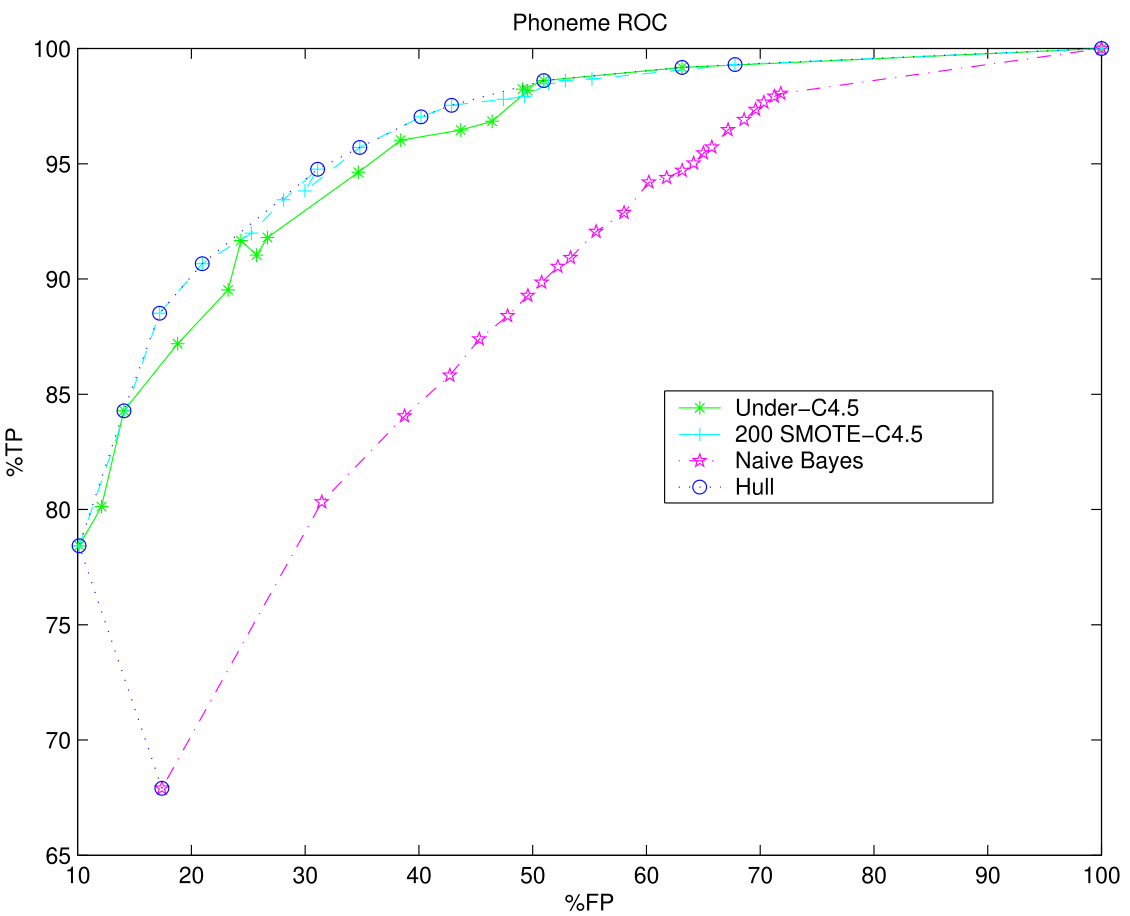
\includegraphics[scale = 1]{ej_smote.png}
	\caption{Comparación de SMOTE con otros métodos de sobremuestreo en el conjunto de datos Phonome. En el eje X los falsos positivos y en el eje Y los verdaderos positivos. Imagen obtenida de \cite{SMOTE}.}
	\label{fig:comparacionSMOTE}
\end{figure}

Como vemos en la figura \ref{fig:comparacionSMOTE}, este método se comporta bastante bien en comparación con otros métodos y es capaz de obtener buenos resultados, sin embargo, tiene algunos problemas.

Uno de estos problemas es que cuando existe ruido entre las clases, o las clases se encuentran dispersas por el espacio de valores, gran parte de los valores sintéticos se encontrarán en una zona del espacio que no corresponde a su clase.

Este problema se hace mucho más presente en nuestro caso, al contar con tantas clases y con tantas características, y para resolverlo se propuso la variante Borderline-SMOTE.

\subsubsection{Borderline SMOTE}


Borderline SMOTE \cite{BL-SMOTE} se trata de una variante de SMOTE que propone buscar los límites en el espacio de valores de la clase a obtener nuevos datos sintéticos, de forma que cuando se generen dichos datos nuevos, estén dentro de dichos límites. De esta forma evitamos problemas con conjuntos de datos con mucho ruido y múltiples clases.

En su artículo proponen dos variantes, una donde las nuevas muestras sintéticas son creadas a partir de todo el conjunto de datos, y otra donde las nuevas muestras solo se generan a partir de los datos considerados en el límite.


\begin{figure}[H]
    \centering
    \begin{subfigure}[b]{0.33\textwidth}
		  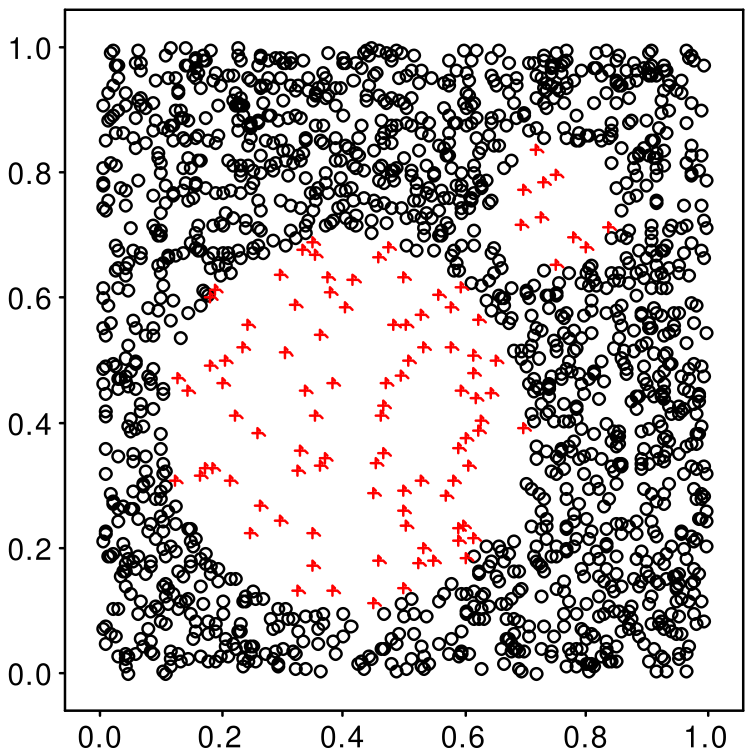
\includegraphics[width=\textwidth]{bl-smote-original.png}
        \caption{}
        \label{fig:blSMOTE-orig}
    \end{subfigure}
    \begin{subfigure}[b]{0.33\textwidth}
        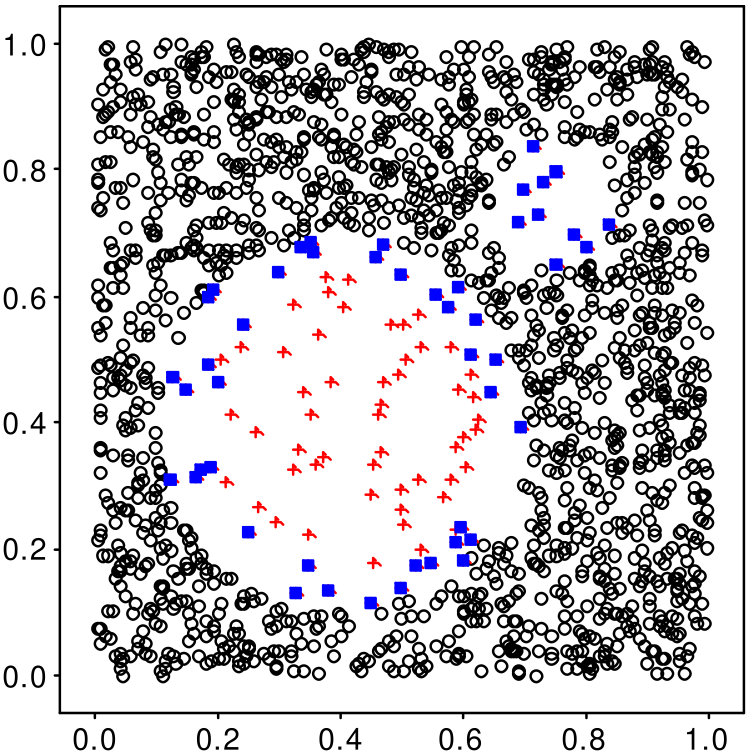
\includegraphics[width=\textwidth]{bl-smote-datos-borderline.png}
        \caption{}
        \label{fig:blSMOTE-border}
    \end{subfigure}
    \begin{subfigure}[b]{0.33\textwidth}
        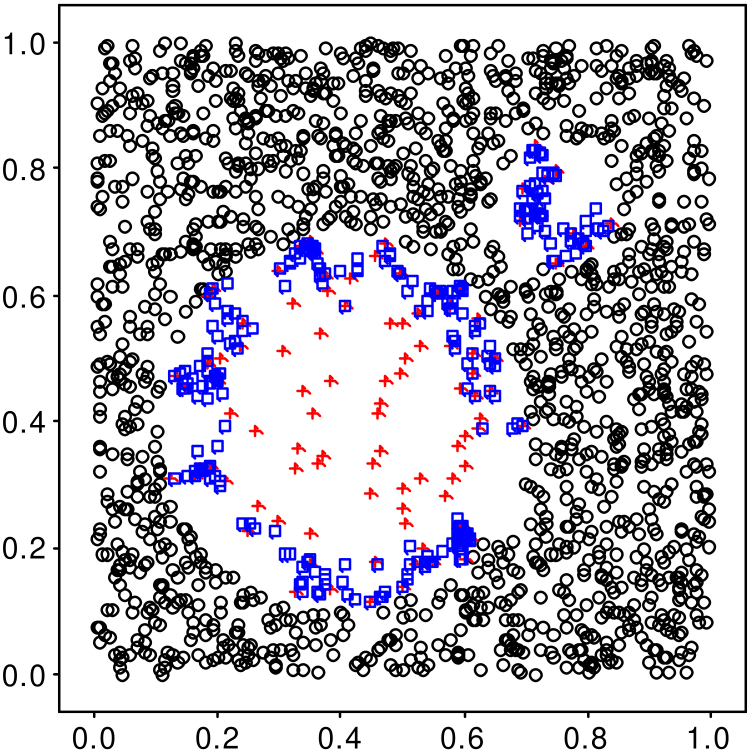
\includegraphics[width=\textwidth]{bl-smote-datos-sinteticos.png}
        \caption{}
        \label{fig:blSMOTE-sintetico}
    \end{subfigure}

    \caption{\ref{fig:blSMOTE-orig} Conjunto de datos original. \ref{fig:blSMOTE-border} datos que conforman el límite de la clase minoritaria (cuadros azules rellenos). \ref{fig:blSMOTE-sintetico} Nuevos datos generados de forma sintética dentro de los límites de la clase (cuadros azules no rellenos). Imagen obtenida de \cite{BL-SMOTE}.}
	 \label{fig:ejemploBL-SMOTE}

\end{figure}


\begin{figure}[H]
    \centering
	 \begin{subfigure}[b]{\textwidth}
		 \centering
		 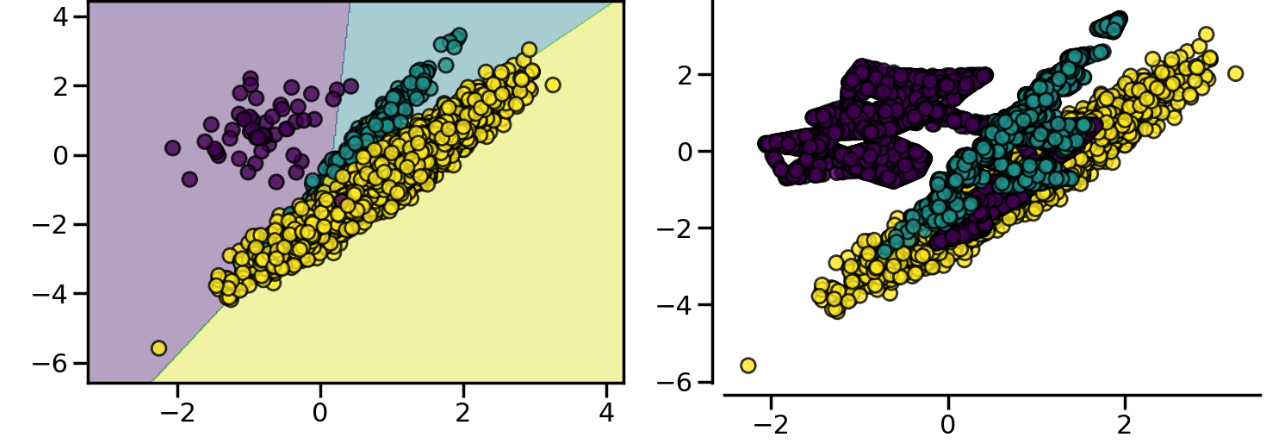
\includegraphics[width=0.8\textwidth]{resampling_smote.png}
		 \caption{A la izquierda bordes de las clases, y a la derecha sobremuestreo con SMOTE}
		 \label{fig:SMOTE-cmp}
	 \end{subfigure}

    \begin{subfigure}[b]{\textwidth}
		 \centering
		  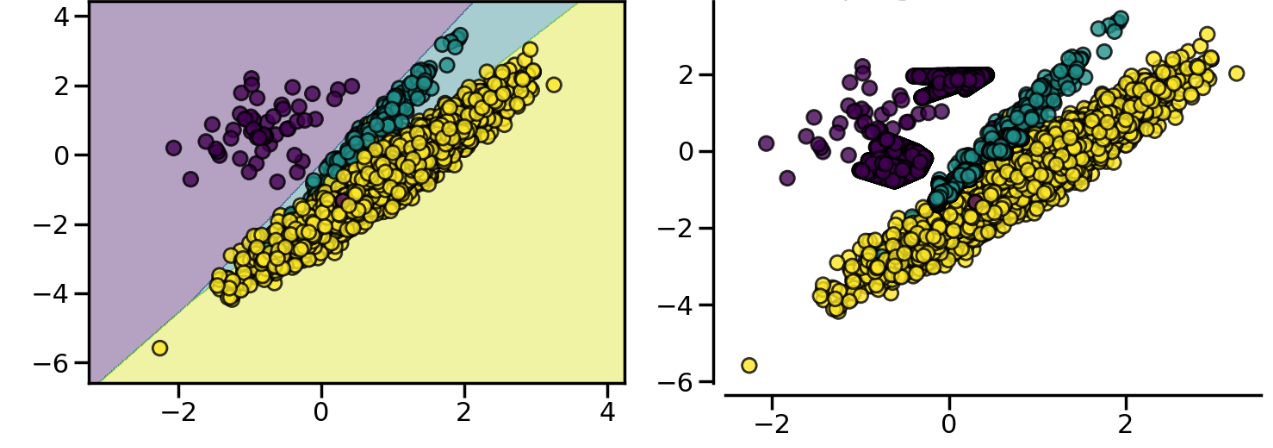
\includegraphics[width=0.8\textwidth]{resampling_blsmote.png}
        \caption{A la izquierda bordes de las clases, y a la derecha sobremuestreo con BorderlineSMOTE}
        \label{fig:BLSMOTE-cmp}
    \end{subfigure}

    \caption{Comparación de SMOTE y BorderlineSMOTE para un conjunto de datos generado aleatoriamente.}\label{fig:BLSMOTE-SMOTE}

\end{figure}

Esta claro que, como vemos en la figura \ref{fig:ejemploBL-SMOTE} y la figura \ref{fig:BLSMOTE-SMOTE}, esta técnica es mucho más versátil y conveniente que SMOTE.


\subsubsection{SMOTER: SMOTE para Regresión}

Uno de los principales problemas que tiene SMOTE es que solo es posible aplicarlo para problemas de clasificación. Para solucionar este problema en 2013 investigadores de la Universidad de Oporto y de Waikato proponen una adaptación del algoritmo SMOTE (o sus variantes) para regresión \cite{SMOTER}.

Este trabajo se centra en resolver tres problemas para poder adaptar SMOTE a un problema de regresión:

\begin{enumerate}
	\item Como definir los datos relevantes y los datos que se consideran raros.
	\item Como crear los nuevos datos sintéticos.
	\item Como asignar un valor numérico a esos datos sintéticos para usarlos en un modelo de regresión.
\end{enumerate}

Con respecto al primer problema, proponen una función de relevancia, en el que el usuario introduzca información sobre que etiquetas hay que obtener nuevos datos, ya que al ser un problema de regresión el número de posibles valores a sobremuestrear es infinito de cara al algoritmo, necesita algo de información sobre que etiquetas es necesario obtener los nuevos datos.

Para resolver el segundo problema proponen generar los datos sintéticos de forma similar al algoritmo SMOTE, adaptando algunos detalles para que sea capaz de trabajar con regresión.

Por último, para tratar el tercer problema, se propone utilizar una media ponderada utilizando el valor de rareza de las etiquetas de los datos con los que se han generado los datos sintéticos.

\begin{figure}[H]
	\centering
	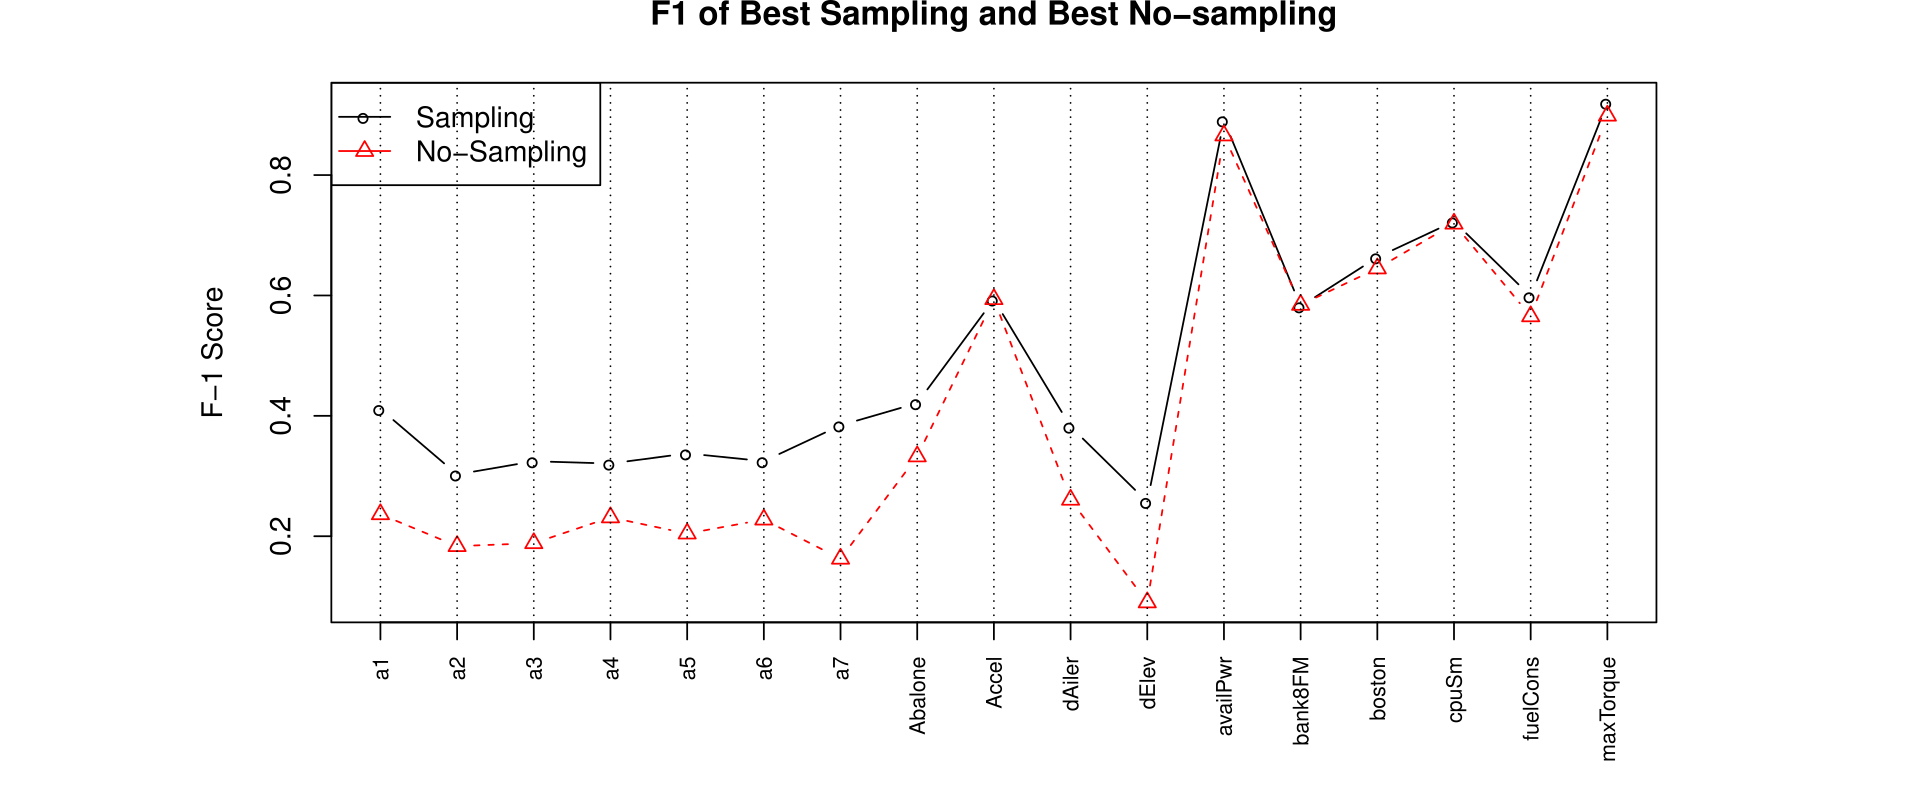
\includegraphics[scale = 1.4]{smoter_resultados.png}
	\caption{Comparación entre un modelo entrenado con los datos originales o los datos sobremuestreados con SMOTER en diecisiete conjuntos de datos. Imagen obtenida de \cite{SMOTER}.}
	\label{fig:smoter_resultados}
\end{figure}

Como vemos, en la mayoría de conjuntos de datos es capaz de mejorar notablemente los resultados, y en ninguna de las pruebas se obtienen peores resultados que en el conjunto de datos original, por lo que vemos que este algoritmo es una buena opción para obtener nuevos datos sintéticos en regresión.

\subsubsection{Algoritmo a utilizar: SMOGN}

SMOGN \cite{SMOGN} se trata de una propuesta publicada en 2017 por los mismos investigadores que propusieron SMOTER. Este trabajo soluciona diversos errores y mejora la propuesta anterior.

En el artículo se describe el problema del balanceo de datos para regresión, así como un análisis de las técnicas utilizadas hasta el momento, como el submuestreo de datos en zonas cuyas etiquetas sean más frecuentes, el uso de SMOTER, o una nueva técnica reciente a la publicación del trabajo basada en introducir nuevas muestras utilizando ruido gaussiano \cite{oversamplingGussianNoise}.

Esta propuesta viene motivada por a dos puntos:

\begin{enumerate}
	\item Limitar los riesgos que asume SMOTER al generar datos sintéticos, ya que descarta los vecinos más alejados y esto puede llevar a generar datos sin apenas muestras.
	\item Aumentar la capacidad de generalización para los casos considerados raros, reduciendo estos casos raros utilizando el ruido gaussiano.
\end{enumerate}

De cara a generar nuevas muestras, SMOGN divide los datos de entrada en dos tipos, casos raros, y por lo tanto relevantes, y casos normales, por lo que no tendrán tanta relevancia ya que el objetivo será crear nuevos datos de los casos considerados raros. Tras esta división, se crearán dos zonas alrededor de donde se quiere crear el nuevo dato sintético, una segura y otra no segura, utilizando umbrales dados por el usuario. Sobre el conjunto de casos relevantes se aplicará SMOTER cuando sea posible y existan vecinos dentro de la zona segura para generar un nuevo dato sintético. Si no hay vecinos en la zona segura, SMOGN estima que no es viable generar el dato con SMOTER, por lo que utilizará ruido gaussiano para generar el dato sintético. Si no es posible generar nuevos datos sintéticos debido a falta de datos originales, se hará un submuestreo en el conjunto de casos normales.


\begin{figure}[H]
    \centering
	  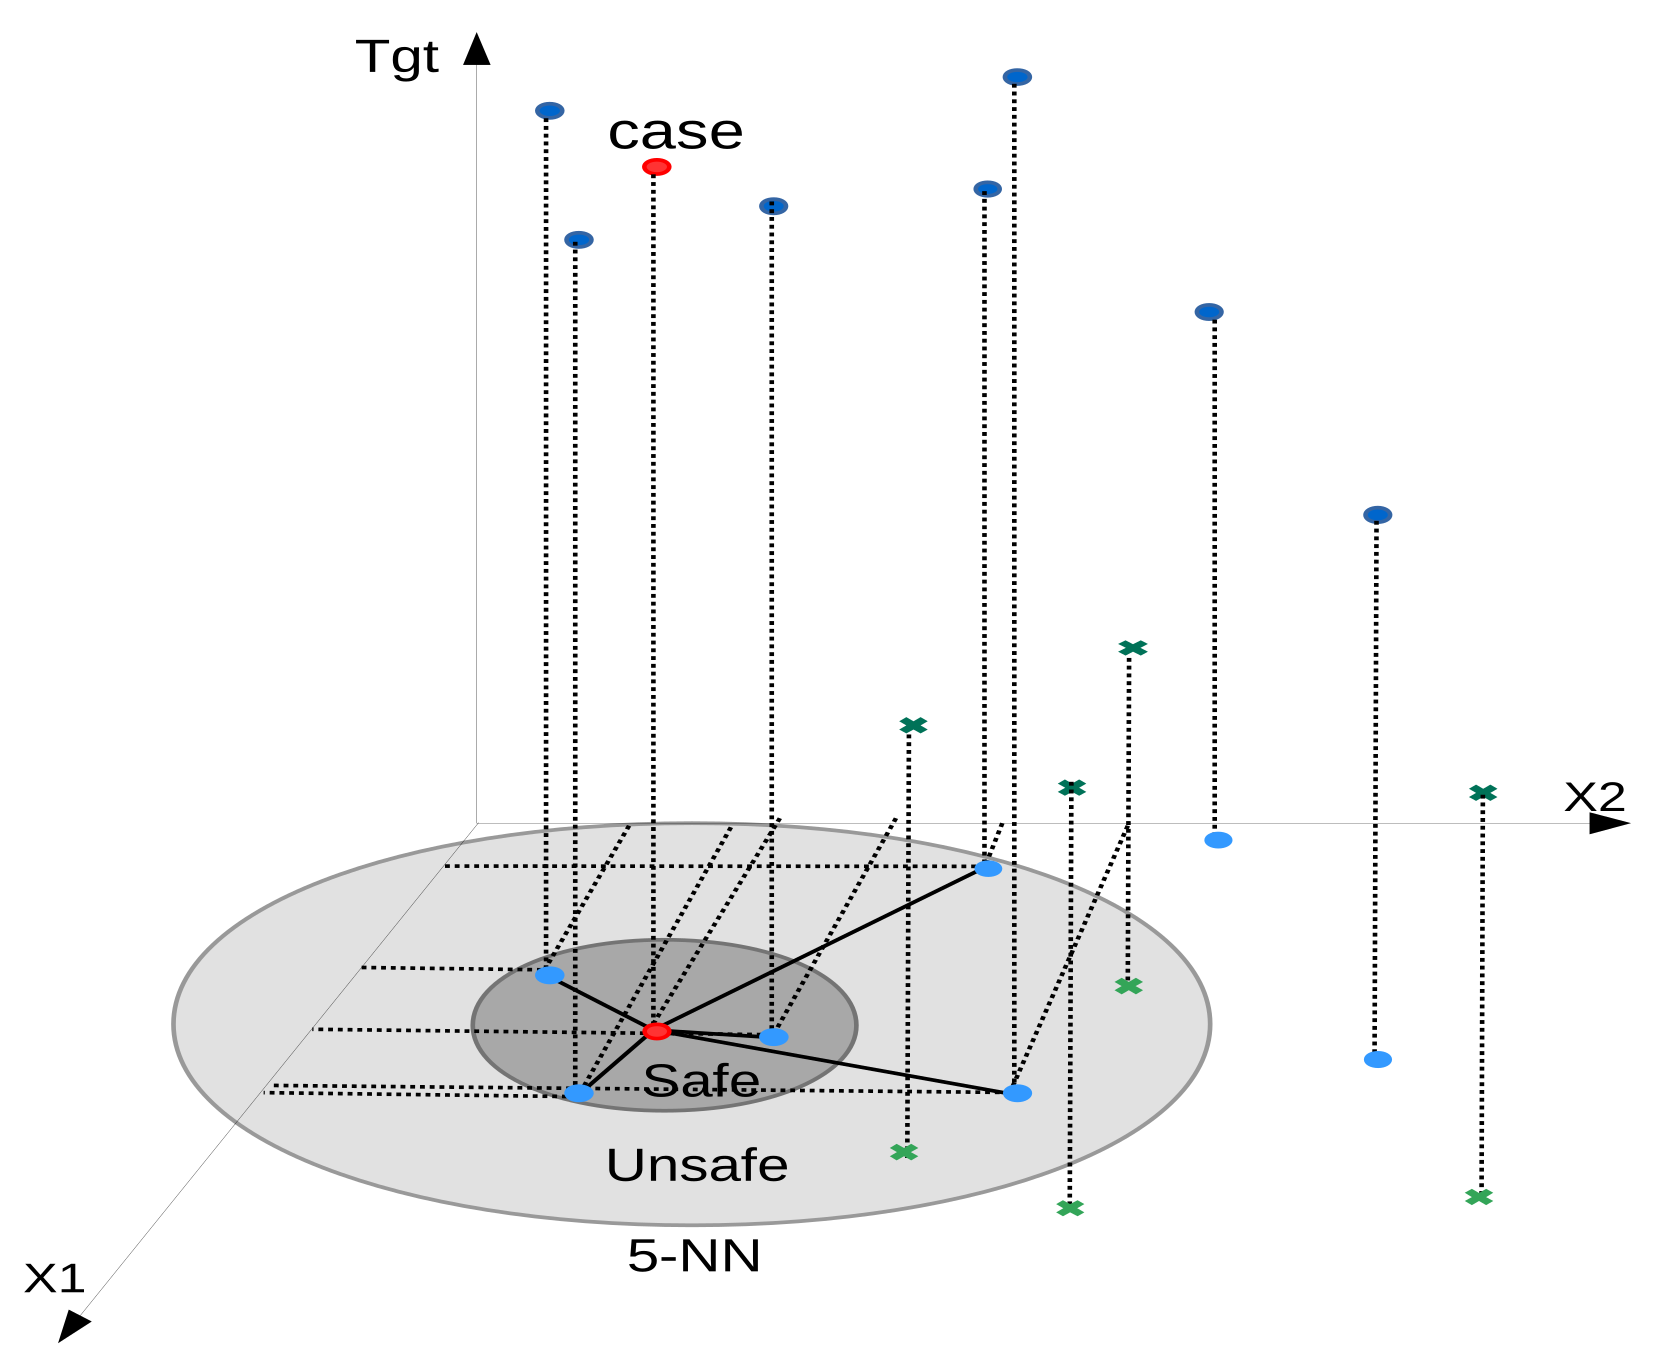
\includegraphics[width=0.6\textwidth]{SMOGN-5NN.png}
    \caption{Ejemplo de un dato sintético generado por SMOGN utilizando los cinco vecinos más cercanos. Imagen obtenida de \cite{SMOGN}}
	 \label{fig:SMOGN-5NN}
\end{figure}


En la figura \ref{fig:SMOGN-5NN} vemos un ejemplo donde los círculos azules son datos considerados relevantes, las cruces verdes datos normales, y se ha creado el nuevo dato en rojo. Podemos distinguir las dos zonas comentadas, segura y no segura, para decidir si aplicar SMOTER o ruido gaussiano. En este caso vemos como si existen una cantidad suficiente de muestras para aplicar SMOTER, luego se escogerá este método para crear el dato. En este ejemplo podemos ver claramente como es mucho más difícil que un dato normal esté en la zona segura, haciendo que SMOTER no obtenga un resultado tan bueno, mientras que si es más común encontrar estos casos en las zonas no seguras, de ahí que en estos casos se utilice el ruido gaussiano.

Finalmente comparan su propuesta con otros métodos como submuestreo aleatorio, introducción de ruido gaussiano, y SMOTER en distintos conjuntos de datos distintos y métodos de entrenamiento distintos, obteniendo finalmente los resultados medios:

\begin{figure}[H]
    \centering
	  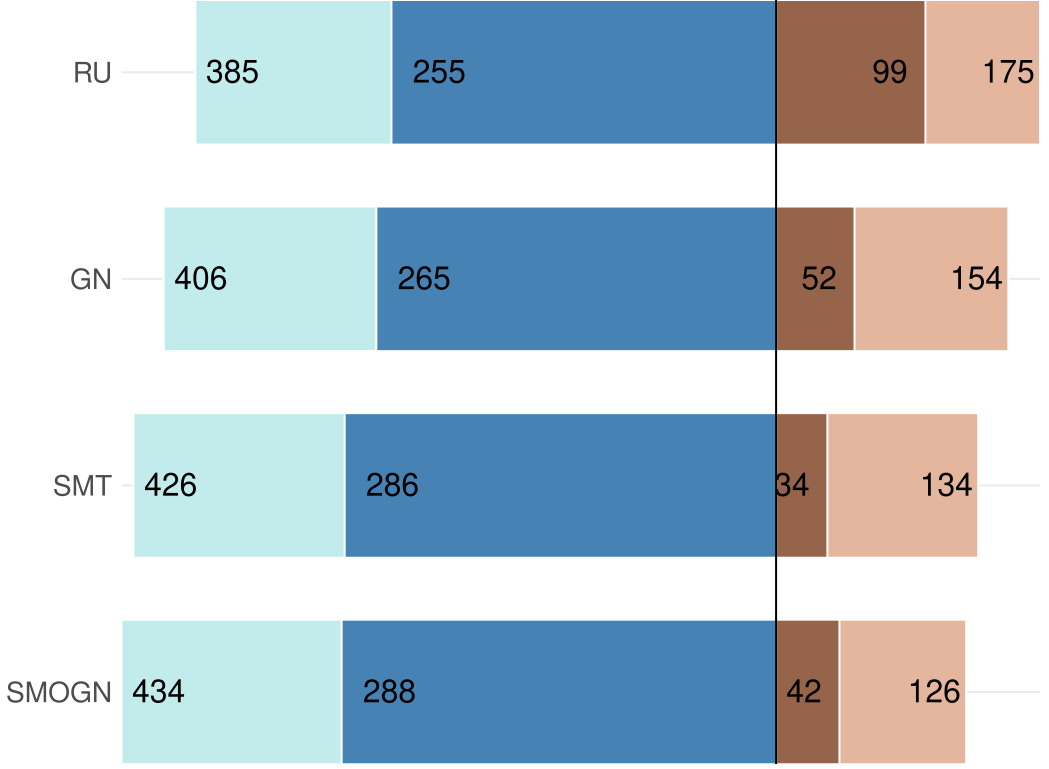
\includegraphics[width=0.5\textwidth]{comparacion_smogn.png}
    \caption{Comparación de SMOGN, Random Undersampling, Gaussian Noise y SMOTER con respecto al conjunto de datos original. A la izquierda número de casos con mejores resultados, y a la derecha peores resultados. Imagen obtenida de \cite{SMOGN}}
	 \label{fig:comparacion_smogn}
\end{figure}

Como nos muestra la figura \ref{fig:comparacion_smogn}, aunque la mayoría de técnicas consiguen mejores resultados que el conjunto de datos original, SMOGN es la que mejores resultados obtiene, minimizando el número de veces en los que no resulta conveniente el sobremuestreo y consiguiendo una amplia ventaja con respecto al conjunto de datos original.


\newpage

\subsection{Resultado tras el preprocesado}

Tras aplicar todas las fases del preprocesado obtenemos los conjuntos de datos finales que utilizaremos.

\begin{figure}[H]
    \centering
	  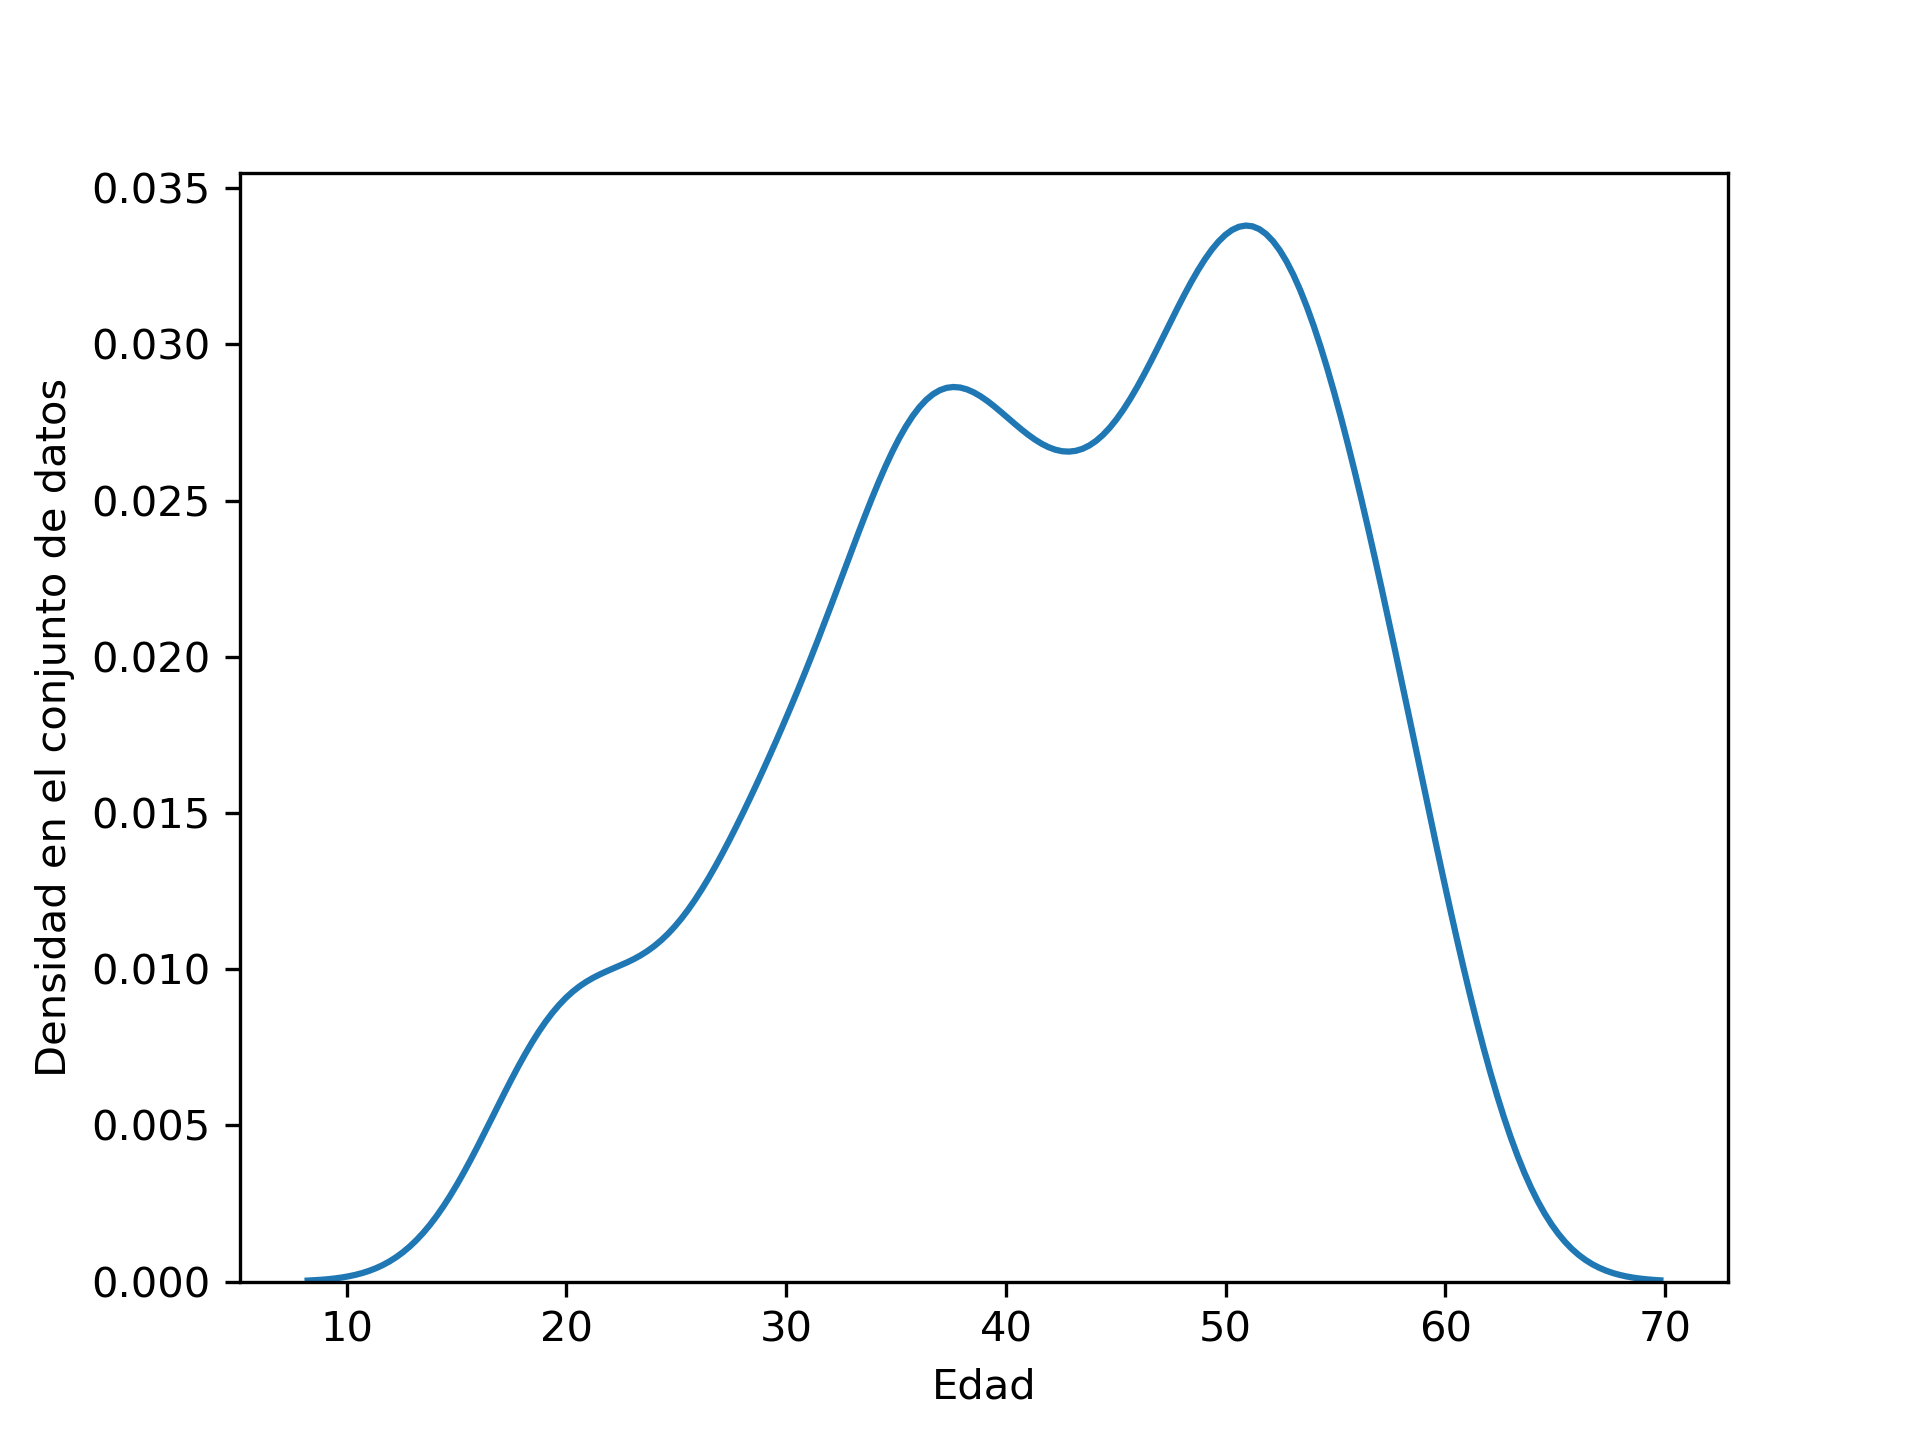
\includegraphics[width=0.6\textwidth]{conjunto_datos/l0_regresion.csv.png}
    \caption{Densidad de cada valor el conjunto de datos original de la lateralidad izquierda.}
	 \label{fig:l0-orig}
\end{figure}

\begin{figure}[H]
    \centering
     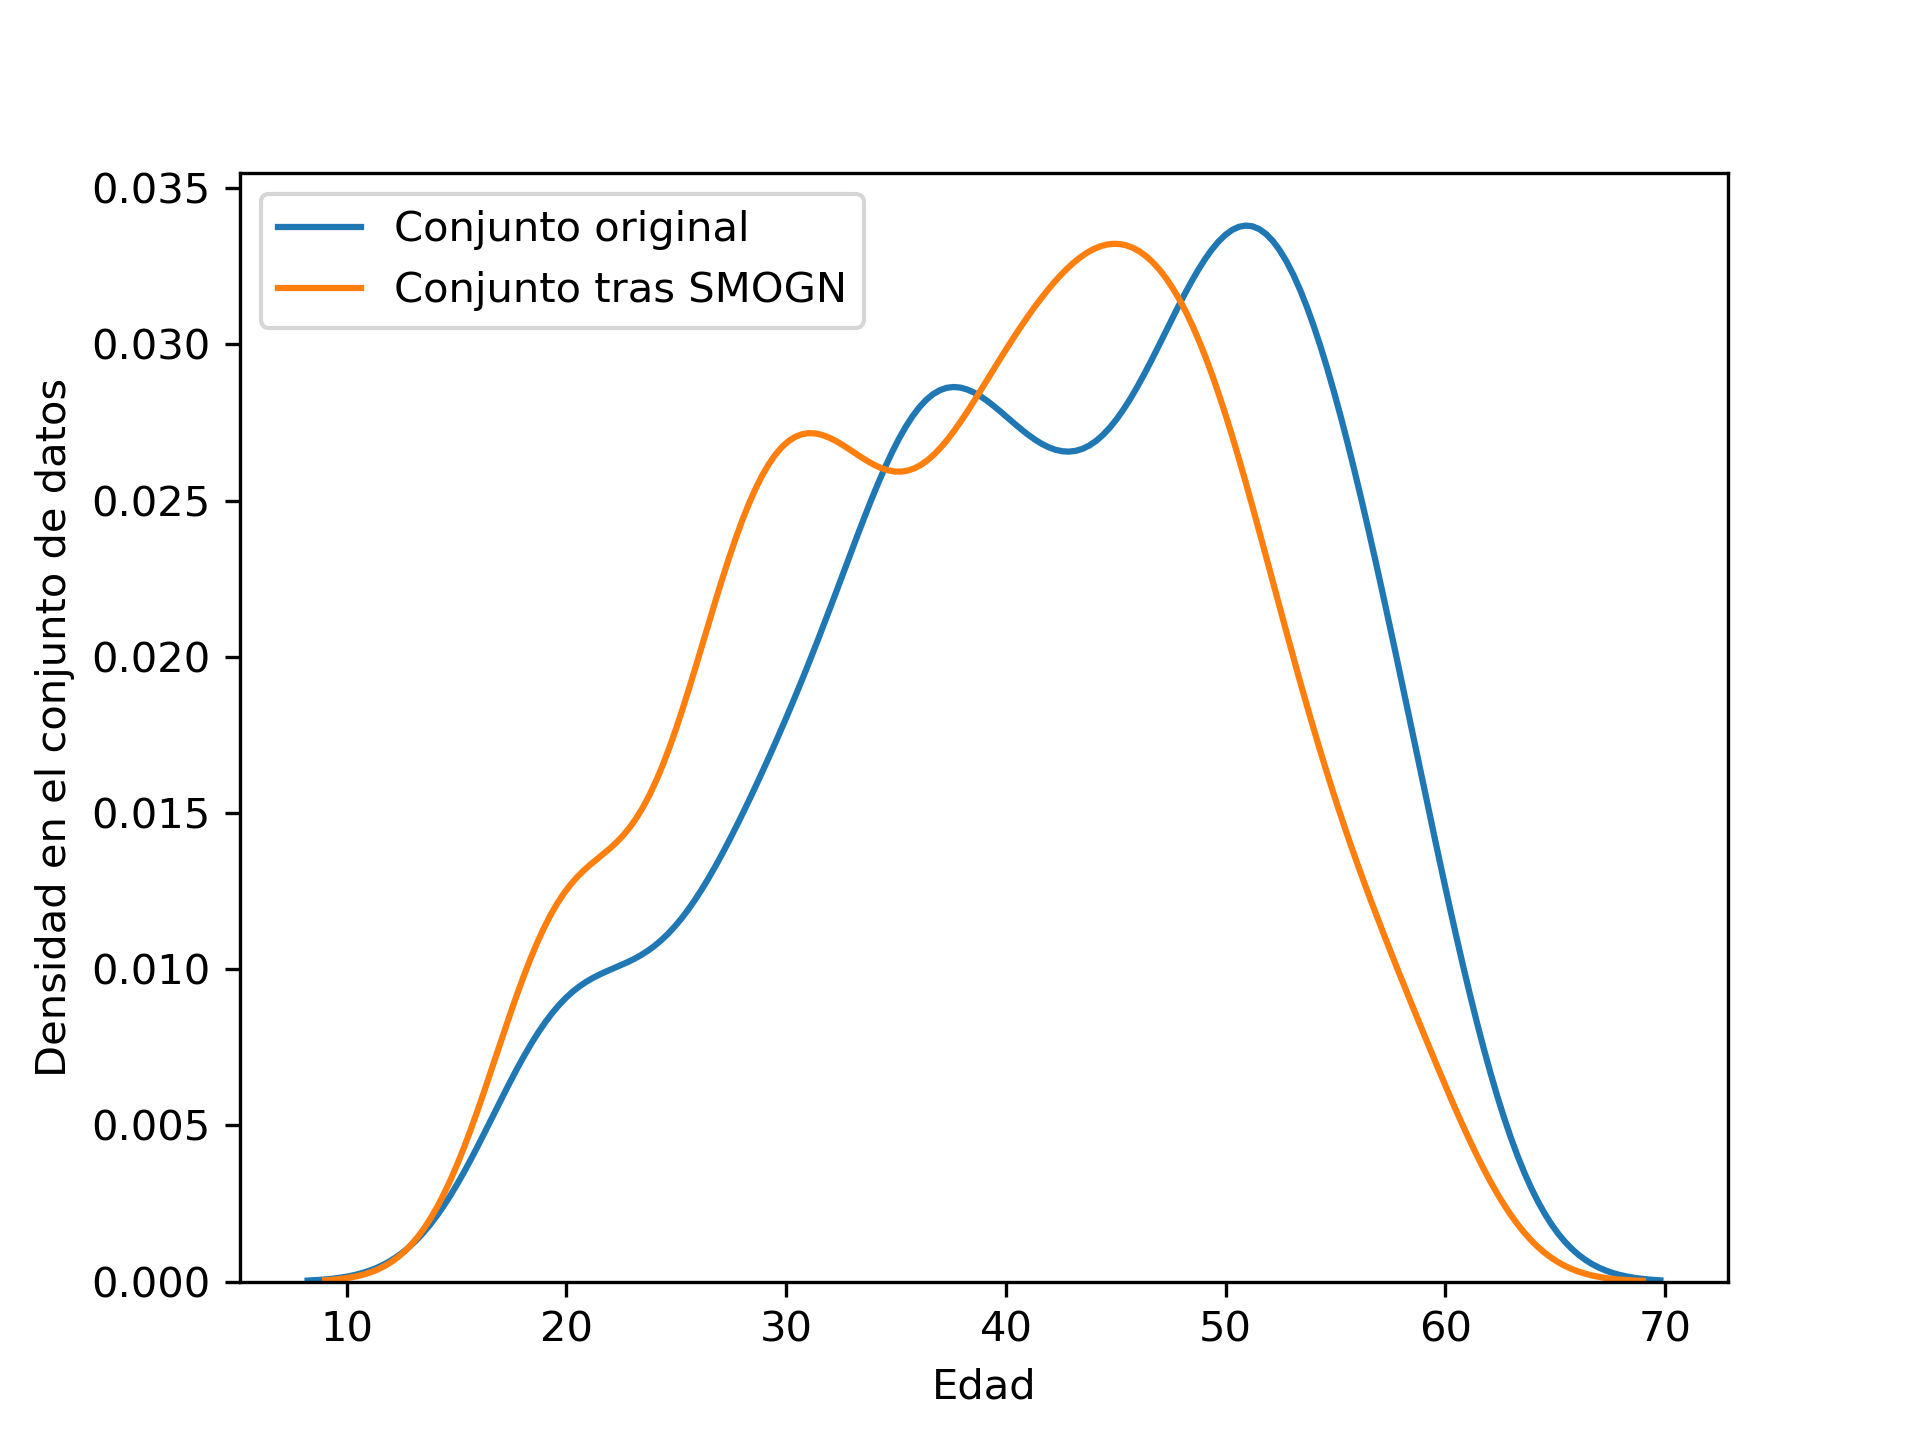
\includegraphics[width=0.6\textwidth]{conjunto_datos/l0_regresion_over_sampling.csv.png}
    \caption{Comparación de la densidad de cada valor el conjunto de datos original de la lateralidad izquierda y tras aplicar SMOGN.}
	 \label{fig:l0-over}
\end{figure}

\begin{figure}[H]
    \centering
	  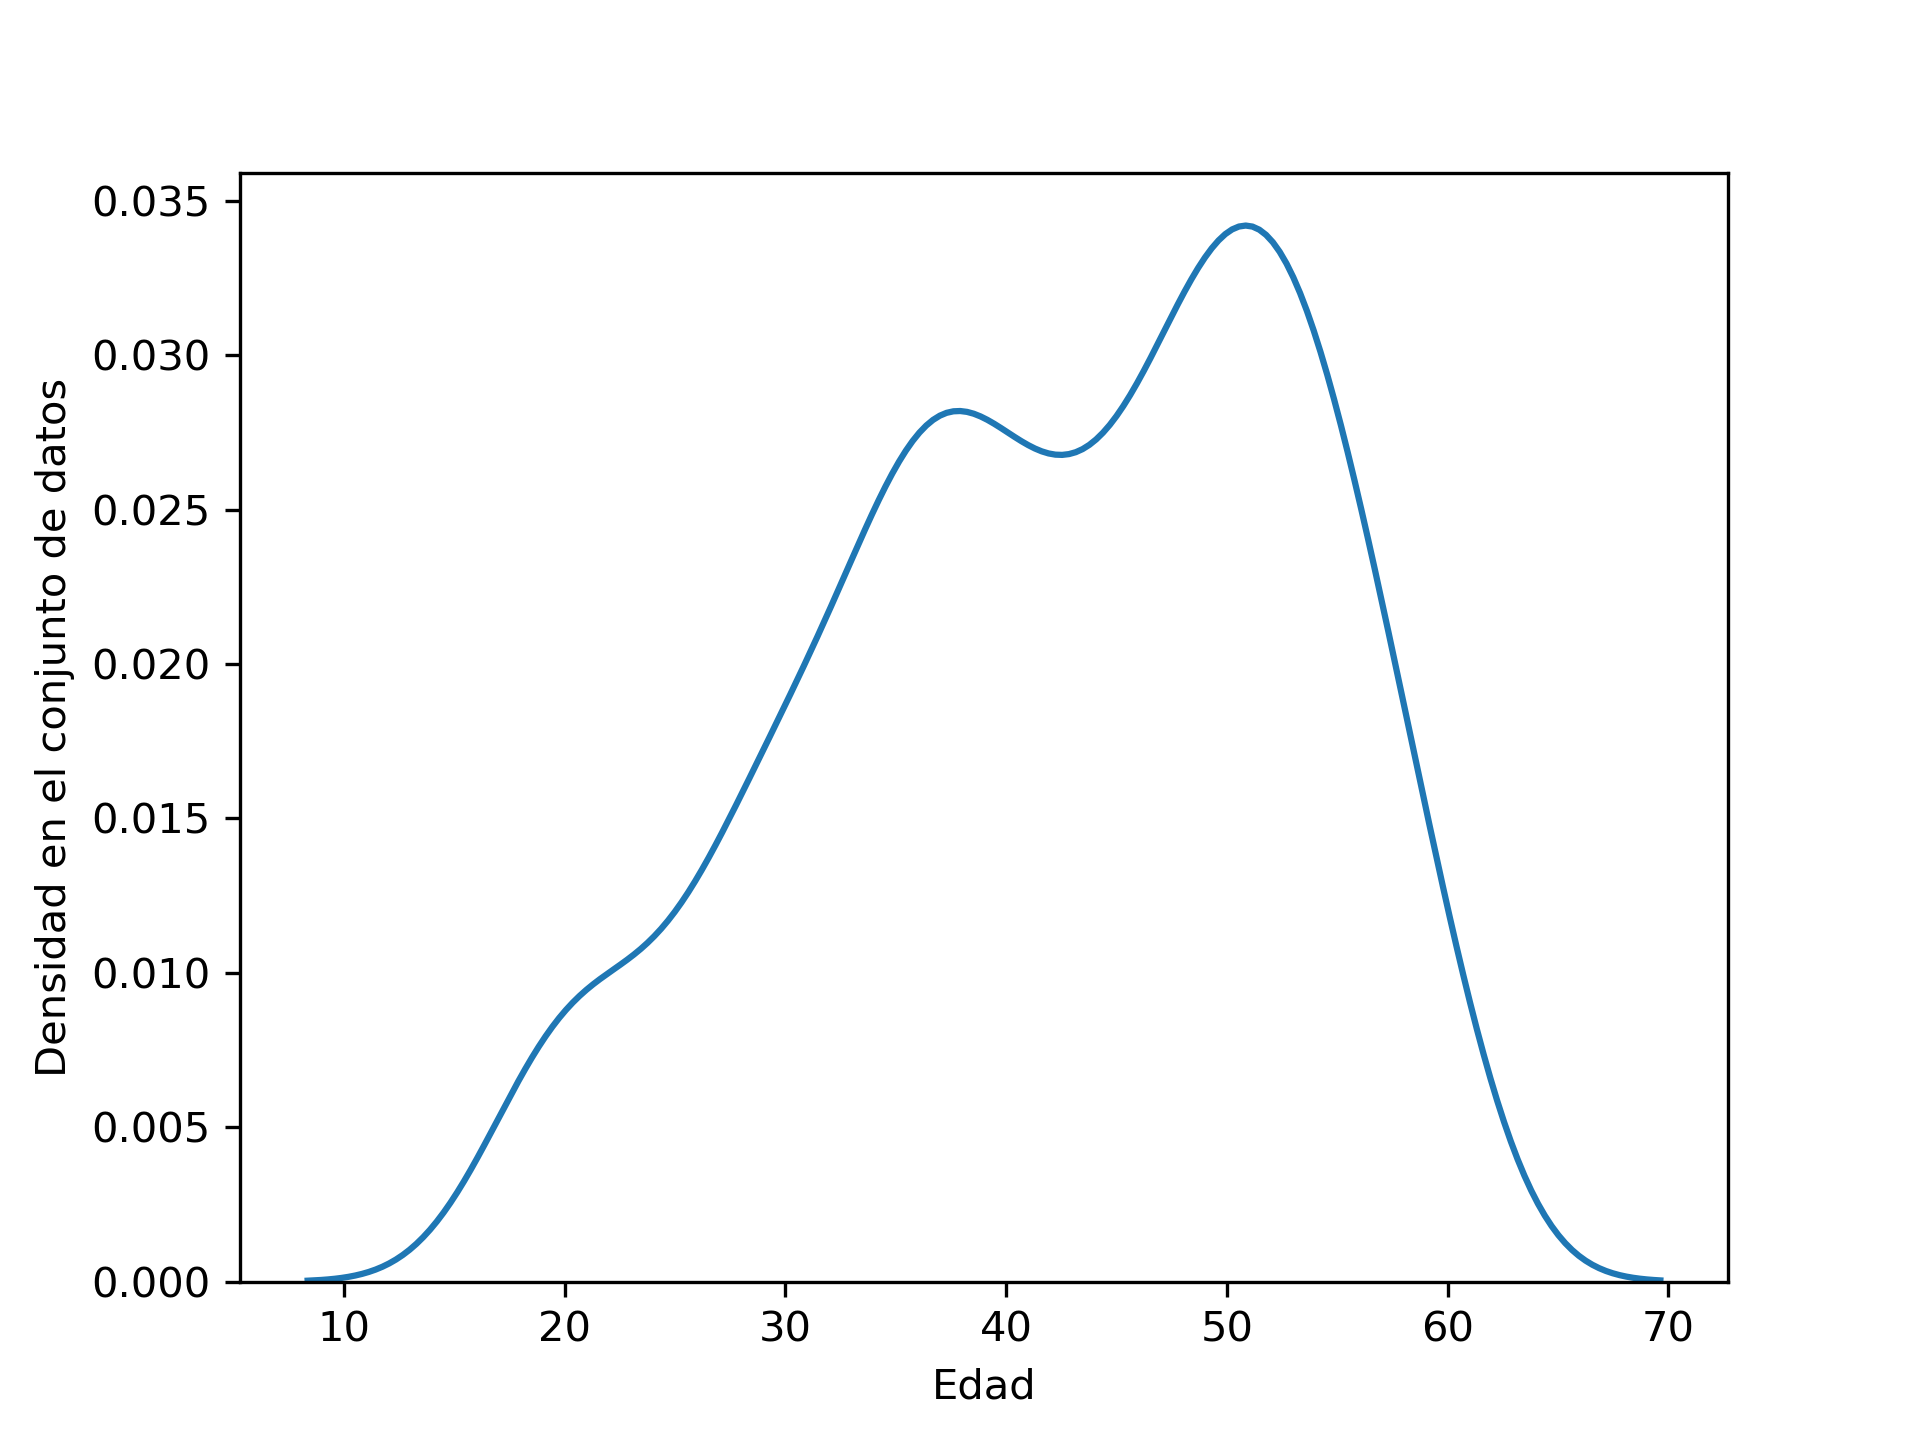
\includegraphics[width=0.6\textwidth]{conjunto_datos/l1_regresion.csv.png}
	  \caption{Densidad de cada valor el conjunto de datos original de la lateralidad derecha.}
	 \label{fig:l1-orig}
\end{figure}

\begin{figure}[H]
    \centering
     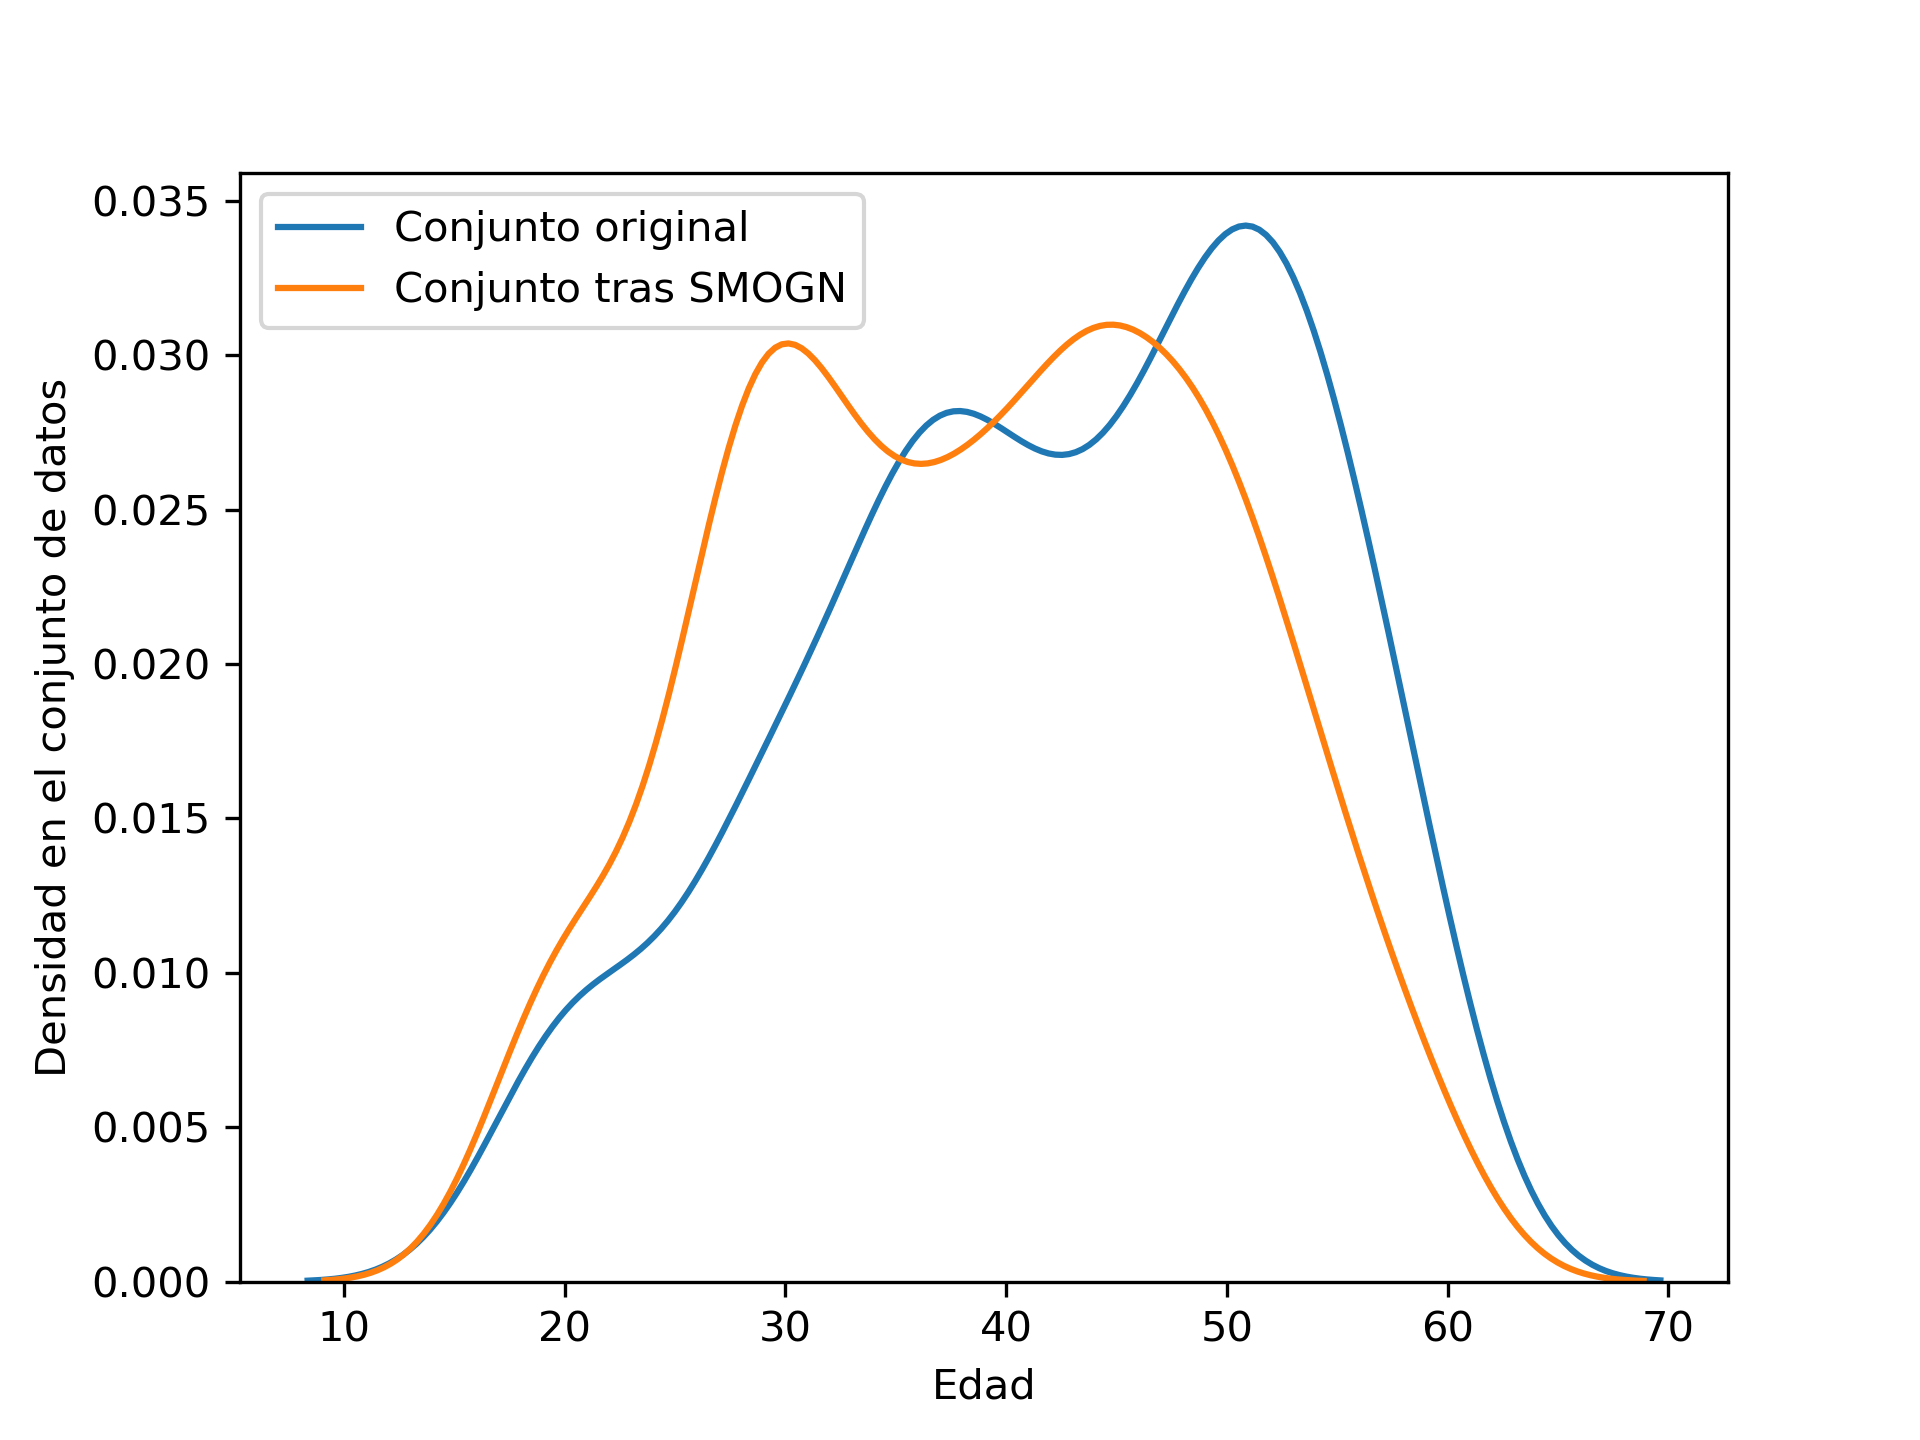
\includegraphics[width=0.6\textwidth]{conjunto_datos/l1_regresion_over_sampling.csv.png}
	  \caption{Comparación de la densidad de cada valor el conjunto de datos original de la lateralidad derecha y tras aplicar SMOGN.}
	 \label{fig:l1-over}
\end{figure}



\begin{figure}[H]
    \centering
	  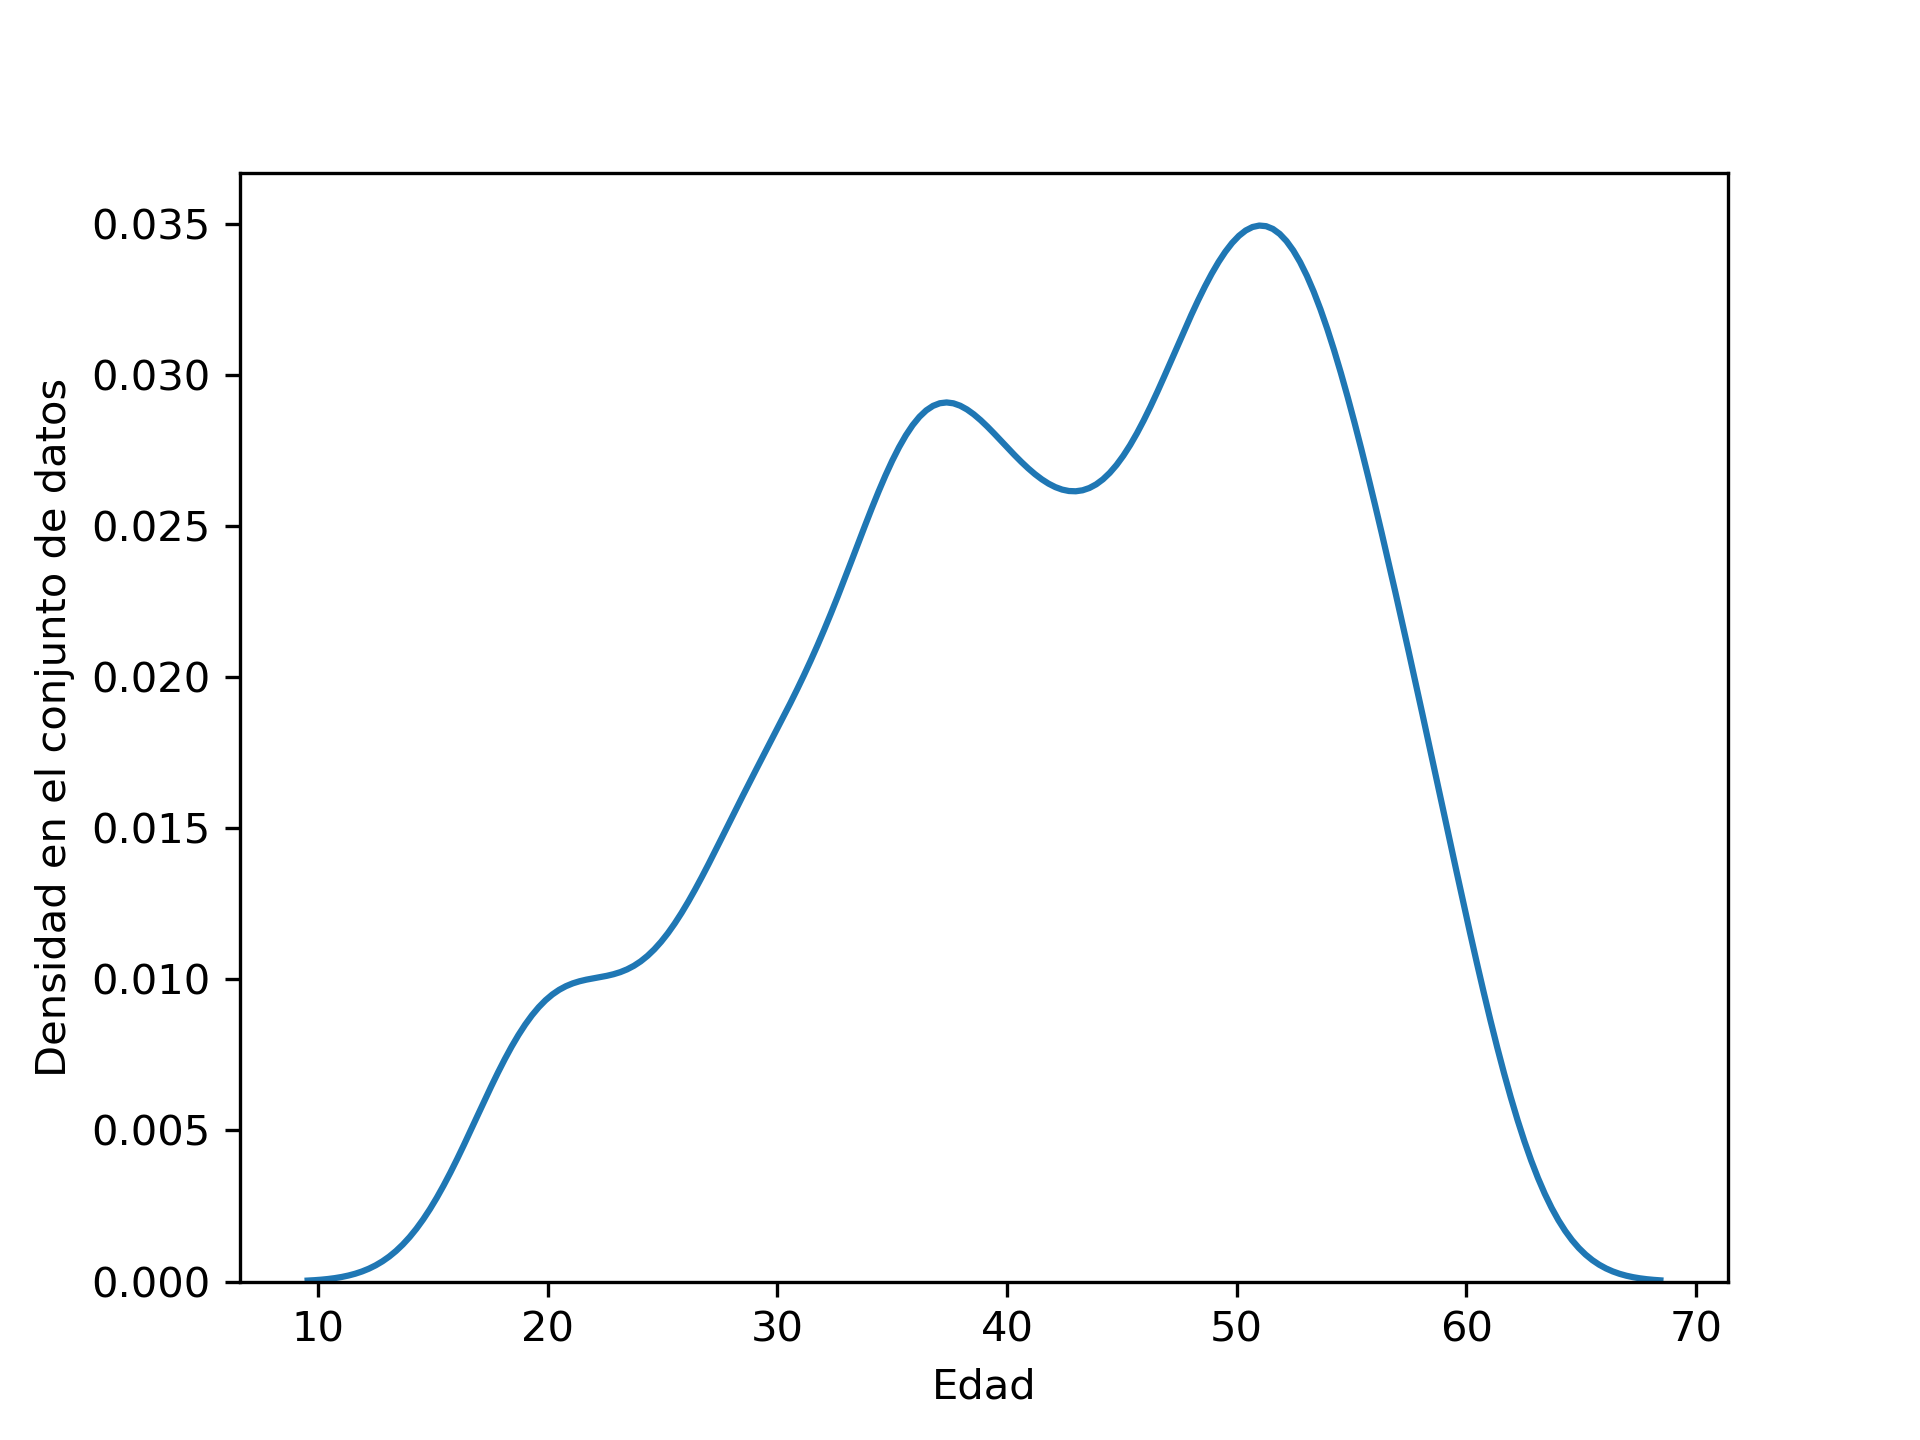
\includegraphics[width=0.6\textwidth]{conjunto_datos/completo_regresion.csv.png}
     \label{fig:completo-orig}
	  \caption{Densidad de cada valor el conjunto de datos original del conjunto completo.}

\end{figure}

\begin{figure}[H]
    \centering
     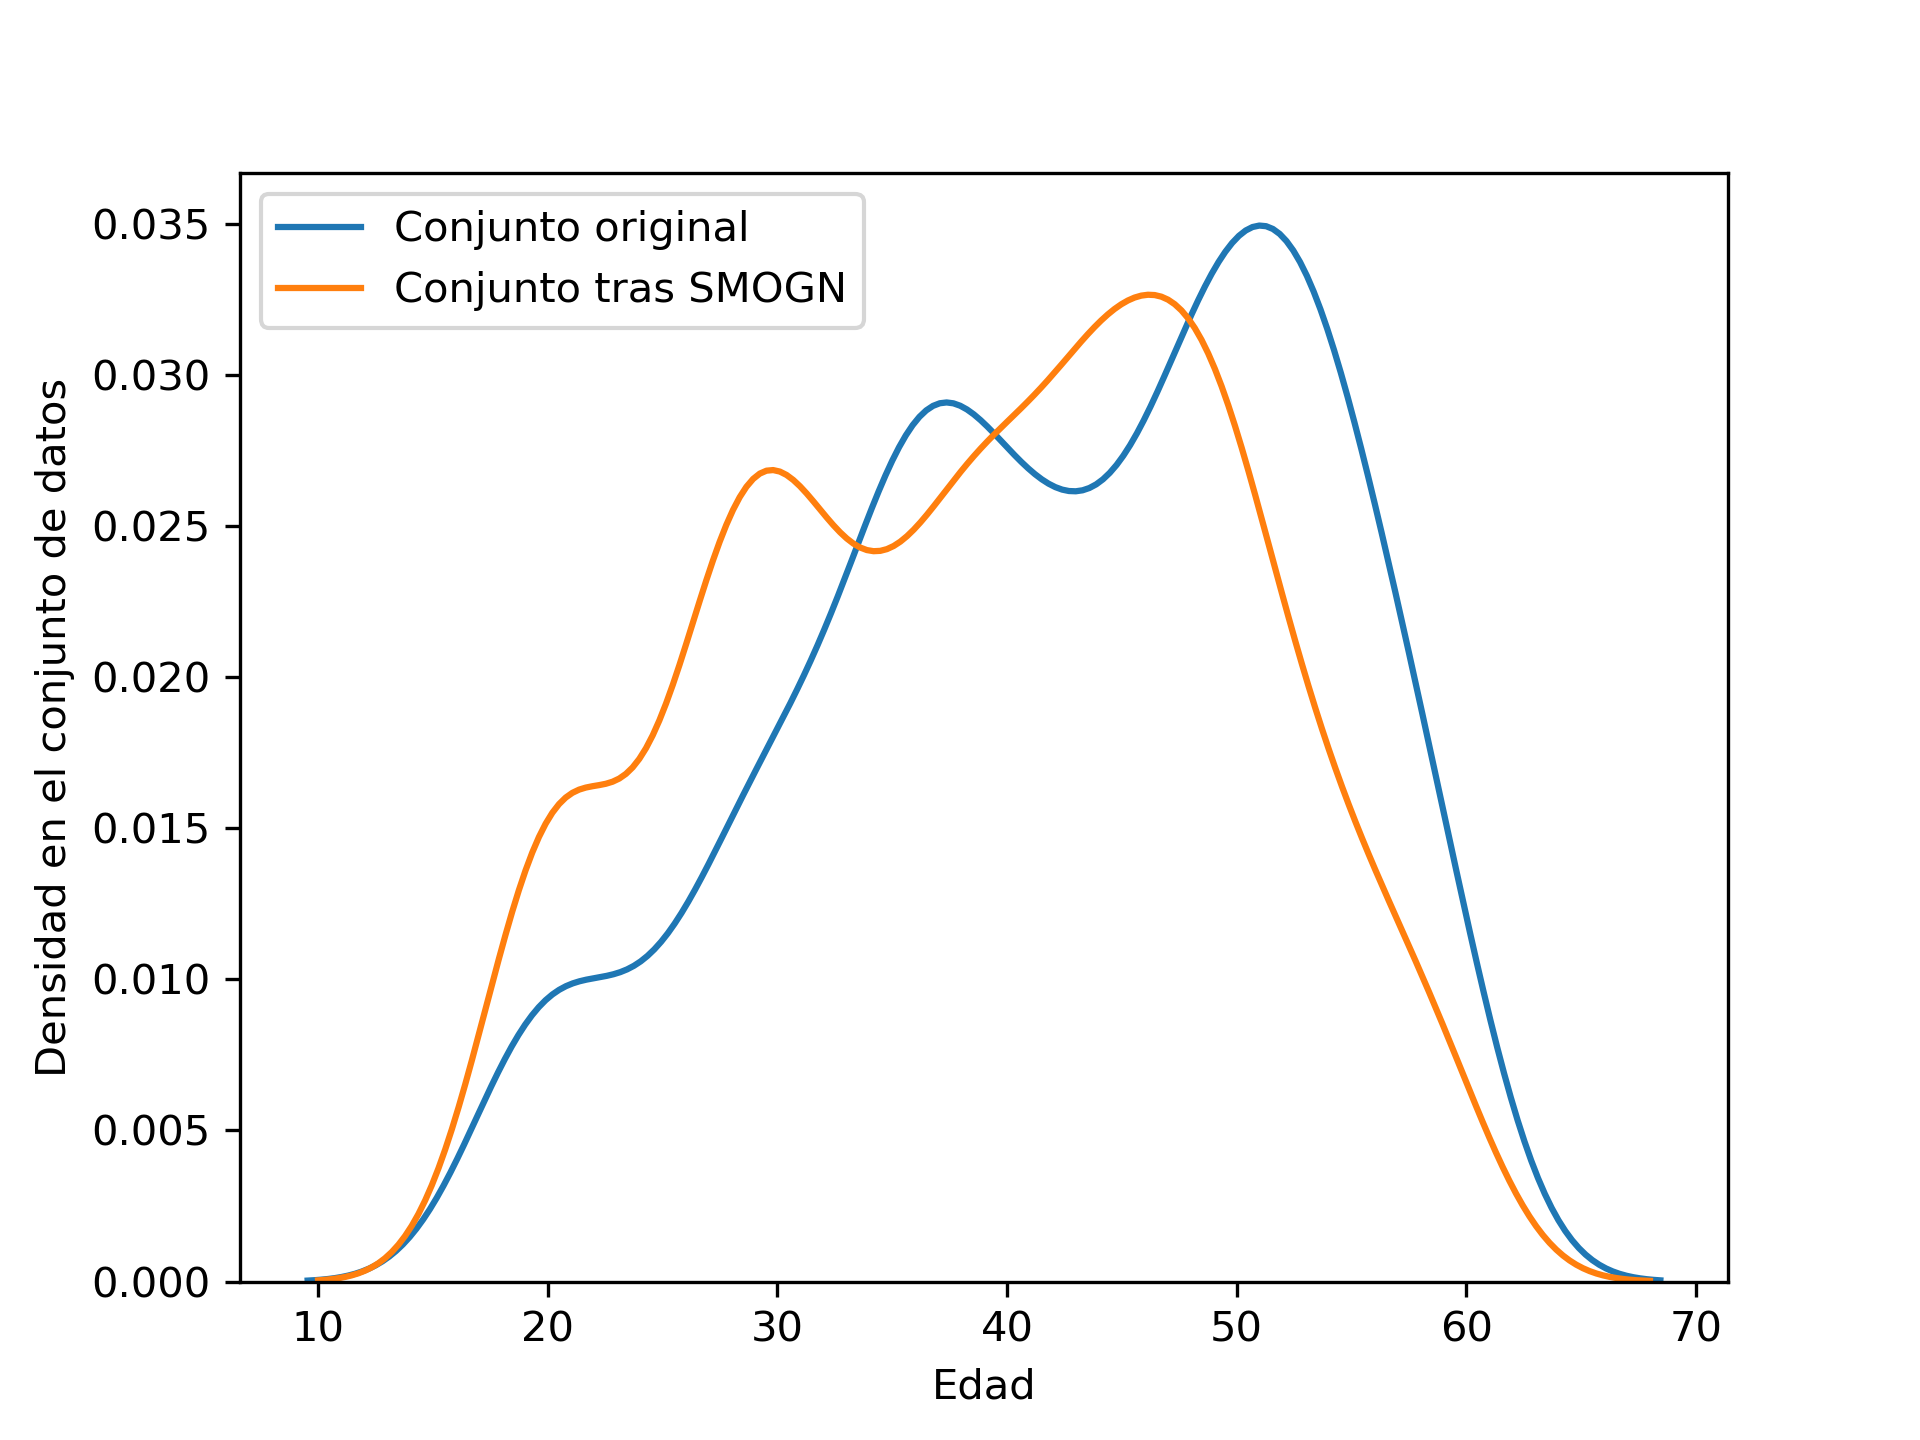
\includegraphics[width=0.6\textwidth]{conjunto_datos/completo_regresion_over_sampling.csv.png}
	  \caption{Comparación de la densidad de cada valor el conjunto de datos original del conjunto completo y tras aplicar SMOGN.}
	 \label{fig:completo-over}
\end{figure}



\begin{table}[H]
\centering
\resizebox{\textwidth}{!}{%
\begin{tabular}{|c|c|c|c|}
\hline
\textbf{}                   & \textbf{Lateralidad izquierda} & \textbf{Lateralidad derecha} & \textbf{Conjunto completo} \\ \hline
\textbf{Original}           & 439                            & 453                          & 892                        \\ \hline
\textbf{Tras aplicar SMOGN} & 579                            & 592                          & 1182                       \\ \hline
\end{tabular}
}
\caption{Comparación del número de datos en el conjunto original y tras aplicar SMOGN.}\label{table:comparacion_orig_SMOGN}
\end{table}

Como vemos en las figuras \ref{fig:l0-over}, \ref{fig:l1-over} y \ref{fig:completo-over} hemos conseguido equilibrar la densidad de las etiquetas, reduciendo la densidad de las etiquetas con valores más altos, los más predominantes en el conjunto de datos, y creando nuevos datos sintéticos de etiquetas con menor valor. Además, como podemos ver en la tabla \ref{table:comparacion_orig_SMOGN}, aumentando el número de muestras, sin necesidad de que SMOGN haya aplicado submuestreo.
